% -*- mode: LaTeX; coding: utf-8 -*-
% Typeset with: XeLaTeX

\documentclass[a4paper,11pt]{article}
\usepackage{a4wide}

% Greek fonts
\RequirePackage{fontspec}
\defaultfontfeatures{Ligatures=TeX}
  % you may want to try: {Liberation Serif} or {Times New Roman}
\setmainfont{FreeSerif}
  % you may want to try: {Liberation Sans} or {Arial}
\setsansfont[Scale=MatchLowercase]{FreeSans}
  % you may want to try: {FreeMono} or {Courier New}
\setmonofont[Scale=MatchLowercase]{FreeMono}

\usepackage{amsmath}
% Required packages for plotting
\usepackage{pgfplots}
%\usepackage{pgfplotstable}
\pgfplotsset{compat=1.16}
%\usepackage{tikz}


\newcommand{\overeq}[1]{\stackrel{\text{#1}}{=}}
\newcommand{\vi}{\mathrm{v}}
\newcommand{\Supp}{\mathrm{Supp}}

% Main document
\begin{document}
\title{Αλγοριθμική Θεωρία Παιγνίων - 1η σειρά ασκήσεων}
\author{Θωμάς Παππάς}
%\date{}
\maketitle

\section*{Πρόβλημα 1}

\begin{enumerate}
	\item Ισχύει\\
	  $\forall t \in S^2$ έχουμε ότι $u_1(A,t)>u_1(C,t)$
	\item Δεν ισχύει\\
	  διότι έχουμε $u_2(D,W) < u_2(D,Z)$
	\item Ισχύει\\
	  $\forall t \in S^2$ έχουμε ότι $u_1(D,t) \geq u_1(B,t)$ με $u_1(D,W)>u_1(B,W)$
	\item Ισχύει\\
	  $\forall s \in S^1$ έχουμε ότι $u_2(W,s)>u_1(Y,s)$ που σημαίνει ότι η $W$ κυριαρχεί αυστηρά την $Y$, άρα και ασθενώς
	\item Ισχύει\\
	  βλέπουμε ότι $u_1(A,W) > \max\{u_1(B,W), u_1(C,W), u_1(D,W)\}$ που σημαίνει ότι η $A$ είναι η μοναδική υποψήφια κυρίαρχη στρατηγική.
	  Όμως $u_1(A,Z) = u_1(D,Z)$ οπότε η $A$ δεν είναι κυρίαρχη και άρα δεν υπάρχει καμία κυρίαρχη στρατηγική για τον παίκτη 1
	\item Δεν ισχύει\\
	  διότι $u_2(A,Y) > u_2(A,Z)$
	\item Ισχύει\\
	  αφαιρούμε τις στρατηγικές $B,C$ και $X,Y$ (κυριαρχούνται αυστηρά από τις $A$ και $W$ αντίστοιχα) και από τα υπόλοιπα σημεία το $(D,Z)$ είναι σημείο ισορροπίας αφού $u_1(D,Z) \geq u_1(A,Z), u_2(D,Z) \geq u_2(D,W)$ και το κοινωνικό όφελος είναι $u_1(D,Z) + u_2(D,Z) = 5+6<13$
\end{enumerate}


\section*{Πρόβλημα 2}

Για αρχή παρατηρούμε αν $a_1=50$ τότε ο π.1 θα πάρει σίγουρα $50$ ευρώ, αφού
\begin{itemize}
	\item αν $a_2 \leq 50$ τότε $u_1(50,a_2) = 50$ (από κανόνα $1$)
	\item αν $a_2 > 50$ τότε $u_1(50,a_2) = 50$ (από κανόνα $3$)
\end{itemize}
που σημαίνει ότι όλες οι στρατηγικές όπου $a_1<50$ κυριαρχούνται αυστηρά από την παραπάνω αφού αν $a_1<50$ τότε $\forall a_2: u_1(a_1,a_2) = a_1 < 50$.
\\
Ομοίως και για τον π.2, που σημαίνει ότι οι στρατηγικές $a_1<50$ και $a_2<50$ μπορούν να αφαιρεθούν με οποιαδήποτε σειρά και χωρίς να επηρεάσουν κάποιο σημείο ισορροπίας.
\newpage
Τώρα αν $a_1=100$ τότε πέρα από την περίπτωση $a_2=100$ όπου θα πάρουν και οι δύο $50$ ευρώ, αν $a_2 \in [51, 99]$ έχουμε $u_2(100,a_2)=a_2>50,u_1(100,a_2)=100-a_2<50$. Οπότε η στρατηγική $a_1=100$ είναι ασθενώς κυριαρχούμενη από την $a_1=50$ και μπορεί να αφαιρεθεί. Προφανώς ομοίως και για τον π.2.
\\[8pt]
Με την ίδια λογική βλέπουμε ότι και οι στρατηγικές $a_1=99$ και $a_2=99$ κυριαρχούνται ασθενώς από τις $a_1=50$ και $a_2=50$ αντίστοιχα (εφόσον έχουμε αφαιρέσει τις $a_1=100$ και $a_2=100$), και αναδρομικά ομοίως για όλες τις στρατηγικές $a_1,a_2 \in [52,100]$. Οπότε οι στρατηγικές που επιβιώνουν είναι οι
\begin{center}
	\begin{tabular}{c || c | c}
		& 50 & 51\\
		\hline\hline
		50 & 50 & 50\\
		51 & 50 & 50
	\end{tabular}
\end{center}
Βλέπουμε όμως ότι πριν αφαιρέσουμε κάποια από τις προηγούμενες ασθενώς κυριαρχούμενες στρατηγικές, έχουμε ότι η $a_1=50$ κυριαρχείται ασθενώς από την $a_1=51$ αφού $u_1(50,52) = 50 < 51 = u_1(51,52)$ (και πάλι ομοίως για τον π.2).
\\[8pt]
Άρα η μοναδική στρατηγική που θα επιβιώσει ανεξάρτητα από τη σειρά με την οποία θα αφαιρέσουμε τις ασθενώς κυριαρχούμενες στρατηγικές είναι η $(51,51)$.


\section*{Πρόβλημα 3}

\paragraph{(i)} Θα πρέπει να ισχύει $\vi_1=\vi_2$, οπότε έχουμε:
\begin{flalign}
  \vi_1=\vi_2 &\Rightarrow \mathrm{max}_i\mathrm{min}_j A_{ij} = \mathrm{min}_j\mathrm{max}_i A_{ij} &\nonumber\\
    &\Rightarrow \max\{\min\{a,5\},1,2\} = \min\{\max\{a,3\},6,7\} \label{eqv}
\end{flalign}
\begin{itemize}
	\item Αν $a > 5$ τότε \eqref{eqv} $\Rightarrow \max\{5,1,2\} = \min\{a,6,7\} \Rightarrow 5 = \min\{a,6\}$ που δεν γίνεται
	\item Αν $3 \leq a \leq 5$ τότε \eqref{eqv} $\Rightarrow \max\{a,1,2\} = \min\{a,6,7\} \Rightarrow a = a$ που ισχύει
	\item Αν $a < 3$ τότε \eqref{eqv} $\Rightarrow \max\{a,1,2\} = \min\{3,6,7\} \Rightarrow \max\{a,2\} = 3$ που δεν γίνεται
\end{itemize}
Οπότε το παίγνιο έχει σημείο ισορροπίας μόνο όταν $a \in [3,5]$.


\paragraph{(ii)} Η αναπαράσταση του παιγνίου είναι η εξής:
\begin{center}
	\begin{tabular}{c || c | c | c | c}
		& Δ1-Μ1 & Δ1-Μ2 & Δ2-Μ1 & Δ2-Μ2\\
		\hline\hline
		Δ1-Μ1 & $0$ & $2$ & $-3$ & $0$\\
		Δ1-Μ2 & $-2$ & $0$ & $0$ & $3$\\
		Δ2-Μ1 & $3$ & $0$ & $0 $& $-4$\\
		Δ2-Μ2 & $0$ & $-3$ & $4$ & $0$
	\end{tabular}
\end{center}
από το οποίο και βλέπουμε ότι αν οι παίκτες επιλέξουν οποιαδήποτε μικτή στρατηγική με Support μόνο τις αμιγείς στρατηγικές Δ1-Μ2 και Δ2-Μ1, τότε το συνολικό τους όφελος θα είναι $0$, και άρα δεν μπορεί να υπάρξει σημείο ισορροπίας σε αυτήν την περίπτωση.\\???


\section*{Πρόβλημα 4}

\paragraph{(i)} Σε ένα $2 \times 2$ παίγνιο, τα πιθανά σημεία ισορροπίας με αμιγείς στρατηγικές είναι τα\\
$(s_1,t_1),(s_1,t_2),(s_2,t_1),(s_2,t_2)$.
Χωρίς βλάβη της γενικότητας, έστω ότι τα $3$ σημεία ισορροπίας είναι τα $(s_1,t_1),(s_1,t_2),(s_2,t_1)$.
Δηλαδή έχουμε:
\begin{flalign}
	&u_1(s_1,t_1) \geq u_1(s, t_1) \forall s \in S \Rightarrow u_1(s_1,t_1) \geq u_1(s_2,t_1) \label{equil1}&\\
	&u_1(s_2,t_1) \geq u_1(s, t_1) \forall s \in S \Rightarrow u_1(s_2,t_1) \geq u_1(s_1,t_1) \label{equil2}\\
	&\eqref{equil1},\eqref{equil2} \Rightarrow u_1(s_1,t_1) = u_1(s_2,t_1) \label{equil3}
\end{flalign}
Τότε $\forall p \in (0,1)$, το προφίλ στρατηγικών $(s^\prime,t_1)$ όπου $s^\prime = (p, 1-p)$ μικτή στρατηγική, είναι επίσης σημείο ισορροπίας, αφού:
\begin{flalign*}
	u_1(s^\prime,t_1) &= p \cdot u_1(e_0,t_1) + (1-p) \cdot u_1(e_1,t_1) = p \cdot u_1(s_1,t_1) + (1-p) \cdot u_1(s_2,t_1) &\\
	  &\overeq{\eqref{equil3}} p \cdot u_1(s_1,t_1) + (1-p) \cdot u_1(s_1,t_1) = u_1(s_1,t_1)
\end{flalign*}
και άρα $u_1(s^\prime,t_1) \geq u_1(e_0,t_1)$ και $u_1(s^\prime,t_1) \geq u_1(e_1,t_1)$.
\\[8pt]
Ομοίως, χρησιμοποιώντας τα σημεία ισορροπίας $(s_1,t_1),(s_1,t_2)$ βρίσκουμε ότι και για τον παίκτη 2, $\forall p \in (0,1)$ το προφίλ στρατηγικών $(s_1,t^\prime)$ όπου $t^\prime = (p, 1-p)$ μικτή στρατηγική, είναι επίσης σημείο ισορροπίας.
\\[8pt]
Συνεπώς (και εφόσον και οποιοσδήποτε συνδυασμός των παραπάνω στρατηγικών επίσης αποτελεί σημείο ισορροπίας) και για τους δύο παίκτες υπάρχει άπειρο πλήθος από σημεία ισορροπίας με μεικτές στρατηγικές.

\paragraph{(ii)} Για αρχή αφαιρούμε την $s_3$ εφόσον κυριαρχείται αυστηρά από τις $s_1,s_2$ και άρα δεν πρόκειται να συμμετέχει σε οποιοδήποτε σημείο ισορροπίας.
\\[8pt]
Μετά κοιτώντας τις αμιγείς στρατηγικές, βλέπουμε ότι το $(s_2,t_1)$ είναι σημείο ισορροπίας, αφού
\[u_1(s_2,t_1) > u_1(s_1,t_1) \text{ και } u_2(s_2,t_1) > u_2(s_2,t_2) > u_2(s_2,t_3)\]
Τέλος για βρούμε αν υπάρχουν μικτές στρατηγικές, έστω $(p,q)$ προφίλ στρατηγικών σε σημείο ισορροπίας, με $p = (p_1,1-p_1)$ και $q = (q_1,q_2,1-q_1-q_2)$.
Οπότε θα πρέπει να ισχύει ότι:
\begin{flalign*}
  u_1(e^1,q) = u_2(e^1,q) &\Rightarrow 0q_1+5q_2+3(1-q_1-q_2) = 2q_1+3q_2+5(1-q_1-q_2) &\\
    &\Rightarrow 5q_2+3-3q_1-3q_2 = 2q_1+3q_2+5-5q_1-5q_2\\
    &\Rightarrow -3q_1-2q_1+5q_1+5q_2-3q_2-3q_2+5q_2 = 5-3\\
    &\Rightarrow 4q_2 = 2 \Rightarrow q_2 = \frac12
\end{flalign*}
\begin{flalign*}
  u_2(p,e^1) &= f_1(p_1) = 0p_1+4(1-p_1) = -4p_1+4 &\\
  u_2(p,e^2) &= f_2(p_1) = 2p_1+3(1-p_1) = -p_1+3\\
  u_2(p,e^3) &= f_3(p_1) = 3p_1+1(1-p_1) = 2p_1+1
\end{flalign*}
Στο τελευταίο κοιτάζουμε τις τιμές που παίρνουν οι $f_1,f_2,f_3$ για $p\in(0,1)$ και παίρνουμε τα σημεία των τομών τους πάνω στη $\max\{f_1,f_2,f_3\}$:

\centering
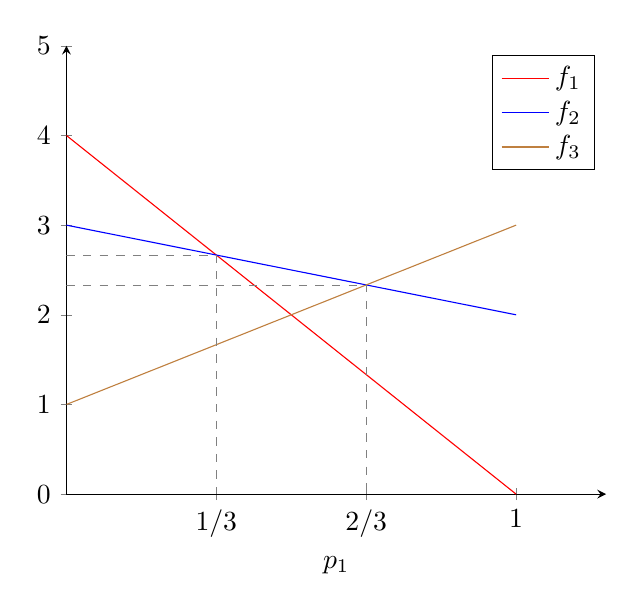
\begin{tikzpicture}
\begin{axis}[
  axis lines=left,
  xmax=1.2, ymax=5,
  xtick={1/3,2/3,1},
  xticklabels={$1/3$,$2/3$,$1$},
  xlabel=$p_1$
]

  % Add all the utility functions.
  \addplot[
    color=red,
    domain=0:1
  ]
  {-4*x+4};
  \addplot[
    color=blue,
    domain=0:1
  ]
  {-x+3};
  \addplot[
    color=brown,
    domain=0:1
  ]
  {2*x+1};
  %\node [fill=black,anchor=center] at (1/3,8/3) {};
  \draw [dashed,help lines] (0,8/3) -| (1/3,0);
  %\node [fill=black,anchor=center] at (2/3,7/3) {};
  \draw [dashed,help lines] (0,7/3) -| (2/3,0);
  \legend{$f_1$,$f_2$,$f_3$}
\end{axis}
\end{tikzpicture}

\raggedright
όπου στα σημεία τομής
\begin{flalign*}
  f_1(p_1) = f_2(p_1) &\Rightarrow -4p_1+4 = -p_1+3 \Rightarrow 3p_1 = 1 \Rightarrow p_1 = \frac13 &\\
  f_2(p_1) = f_3(p_1) &\Rightarrow -p_1+3 = 2p_1+1 \Rightarrow 3p_1 = 2 \Rightarrow p_1 = \frac23
\end{flalign*}
Στην πρώτη περίπτωση όπου $\Supp(q)=\{1,2\}$ έχουμε ότι $q = (1-q_2,q_2,0) \stackrel{q_2=1/2}{=} \left(\frac12,\frac12,0\right)$,\\
ενώ στη δεύτερη όπου $\Supp(q)=\{2,3\}$ έχουμε ότι $q = (0,q_2,1-q_2) \stackrel{q_2=1/2}{=} \left(0,\frac12,\frac12\right)$.
\\[10pt]
Οπότε εντέλει τα σημεία ισορροπίας στο παίγνιο είναι τα
\[(s_2,t_1) = (e^2,e^1), \left(\left(\frac13,\frac23\right),\left(\frac12,\frac12,0\right)\right), \left(\left(\frac23,\frac13\right),\left(0,\frac12,\frac12\right)\right)\]


\section*{Πρόβλημα 5}

Ορίζουμε...
\newpage

\section*{Πρόβλημα 6}

Θα δείξουμε ότι δεν ξέρουμε αν υπάρχει πολυωνυμικός αλγόριθμος για πεπερασμένα παίγνια μηδενικού αθροίσματος με $3$ παίκτες, δείχνοντας ότι ένας τέτοιος αλγόριθμος θα έλυνε και ένα γενικό παίγνιο με $2$ παίκτες.
\\[8pt]
Έστω λοιπόν $G_1$ ένα γενικό παίγνιο $2$ παικτών με στρατηγικές $S^1,S^2$ και utility functions $u_1, u_2$.
Κατασκευάσουμε τώρα ένα παίγνιο $G_2$ από το $G_1$ αλλά με $3$ παίκτες, στρατηγικές $S^1,S^2,S^3$ όπου $S^3 = \{r\}$ (δηλαδή ο π.3 έχει μόνο μία διαθέσιμη στρατηγική) και utility functions $u_1^\prime, u_2^\prime, u_3^\prime$ όπου:
\begin{align}
  u_1^\prime(p,q,r) &= u_1(p,q) \label{nash1}&\\
  u_2^\prime(p,q,r) &= u_2(p,q) \label{nash2}\\
  u_3^\prime(p,q,r) &= -u_1(p,q)-u_2(p,q) \nonumber
\end{align}
Τότε το $G_2$ είναι παίγνιο μηδενικού αθροίσματος με $3$ παίκτες και έχουμε ότι ένα προφίλ στρατηγικών $(p,q)$ είναι σημείο ισορροπίας για το $G_1$ αν και μόνον αν το $(p,q,r)$ είναι σημείο ισορροπίας στο $G_2$.
Όντως για ένα τέτοιο σημείο $(p,q,r)$ και $\forall p^\prime \in S^1, \forall q^\prime \in S^2$ έχουμε ότι:
\begin{itemize}
	\item $u_1(p,q) \geq u_1(p^\prime,q) \stackrel{\eqref{nash1}}{\Leftrightarrow} u_1^\prime(p,q,r) \geq u_1^\prime(p^\prime,q,r)$
	\item $u_2(p,q) \geq u_2(p,q^\prime) \stackrel{\eqref{nash2}}{\Leftrightarrow} u_2^\prime(p,q,r) \geq u_2^\prime(p,q^\prime,r)$
\end{itemize}
Ενώ για τον π.3 στο $G_2$ κάθε σημείο είναι ισορροπίας για αυτόν αφού $|S^3|=1$.
\\[8pt]
Από το παραπάνω βλέπουμε ότι ένα παίγνιο $2$ παικτών μπορεί να αναχθεί σε μια ειδική περίπτωση ενός παιγνίου μηδενικού αθροίσματος $3$ παικτών, και άρα το τελευταίο είναι τουλάχιστον όσο δύσκολο όσο το πρώτο.
Πιο συγκεκριμένα δηλαδή η επίλυση ενός παιγνίου μηδενικού αθροίσματος $3$ παικτών είναι PPAD-hard πρόβλημα, και άρα δεν γνωρίζουμε για την ύπαρξη πολυωνυμικού αλγορίθμου που να το επιλύνει.

\end{document}
